\documentclass{article}
\usepackage{amssymb,amsfonts,amsmath,calc,tikz,geometry}
\usepackage{color}   %May be necessary if you want to color links
\usepackage{hyperref}
\usepackage{amsthm}
\hypersetup{
    colorlinks=false, %set true if you want colored links
    linktoc=all,   %set to all if you want both sections and subsections linked
    linkcolor=black,  %choose some color if you want links to stand out
}
%%%%%%%%%%%%%%%%%%%%%%%%%%%%%%%%%%%%%%%%%%%%%%%%%%%%%%%%%%%%%%%%%%%%%%%%%%%%%%%
\geometry{margin=1in}
\theoremstyle{plain}
\newtheorem{theorem}{Theorem}[section]
\newtheorem{lemma}[theorem]{Lemma}
\newtheorem{proposition}[theorem]{Proposition}
\newtheorem{corollary}[theorem]{Corollary}
\newtheorem{definition}{Definition}[section]
\newtheorem{remark}{Remark}[section]
\DeclareMathOperator{\lcm}{lcm}
\DeclareMathOperator{\idealin}{\triangleleft}
\DeclareMathOperator{\im}{im}
\DeclareMathOperator{\Aut}{Aut}
\DeclareMathOperator{\End}{End}
\DeclareMathOperator{\Inn}{Inn}
\DeclareMathOperator{\Out}{Out}
\DeclareMathOperator{\Mat}{Mat}
\DeclareMathOperator{\std}{std}
\newcommand{\N}{\mathbb{N}}
\newcommand{\Z}{\mathbb{Z}}
\newcommand{\Q}{\mathbb{Q}}
\newcommand{\R}{\mathbb{R}}
\newcommand{\C}{\mathbb{C}}
\newcommand{\F}{\mathbb{F}}
\newcommand{\Omicron}{O}
\newcommand{\bigslant}[2]
{{\raisebox{.2em}{$#1$}\left/\raisebox{-.2em}{$#2$}\right.}}
\newcommand{\ideal}[1]
{\langle $#1$ \rangle}
%%%%%%%%%%%%%%%%%%%%%%%%%%%%%%%%%%%%%%%%%%%%%%%%%%%%%%%%%%%%%%%%%%%%%%%%%%%%%%%
\title{\textbf{Practice}}
\author{Yeheli Fomberg}
\date{326269651}
\begin{document}
	\maketitle
	\newpage
	\section{Rings}
	\textbf{Let $R$ be an integral domain with a multiplicative identity. 
	Find all the units of the polynomials ring: $R[x]$} \\
	We are looking for:
	\[
		\{a \in R[x] \vert \text{$a$ is a unit in $R[x]$}\}
	\]
	We can notice that for two polynomials $p(x)$, $q(x)$ that:
	\[
		\deg(pq) = \deg p + \deg q
	\]
	Let $q$ be a unit in $R[x]$ and $p$ be it's inverse then:
	\[
		0 = \deg(1) = \deg(pq) = \deg p + \deg q
	\]
	This means that:
	\[
		\deg p + \deg q = 0
	\]
	And since a degree of a polynomial must be a natural number the result
	is that all units are exactly the units in $R$ so the set is:
	\[
		\{a \in R[x] \vert \text{$a$ is a unit in $R$}\}
	\]
	
	\newpage
	
	\textbf{Find an invertible polynomial $P$ in $Z_4[x]$ with $\deg P=1$} \\
	We want to find a unit $P$ of $Z_4[x]$, with $\deg P = 1$. Let 
	$P = p_0 + p_1x$
	and let its inverse be 
	$Q = q_0+q_1x$ 
	since we don't need to raise the degree of $P$ over $3$ we may assume 
	$\deg Q = 2$ then:
	\[
		(p_0+p_1x)(q_0+q_1x) = p_0q_0 + (p_0q_1+p_1q_0)x + p_1q_1x^2
	\]
	We want $p_1q_1 = 0$ but since $p_1 \neq 0$ let us choose $p_1=q_1=2$.
	Now we get:
	\[
		(p_0+2x)(q_0+2x) = p_0q_0 + 2(p_0+q_0)x
	\]
	So we need $p_0+q_0=0$ or $p_0+q_0=2$ and $p_0q_0 = 1$. That means we can
	choose $p_0=q_0=1$, and indeed:
	\[
		PQ = (1+2x)(1+2x) = 1 + 4x + 4x^2 = 1
	\]
	Since $P=Q$ it's clear that $PQ=QP=1$ which completes the proof that 
	$2x+1$ is a unit in $\Z_4[x]$, with $\deg (1+2x) = 1$
	
	\newpage
	
	\textbf{Let $R$ be a ring with a unit, and let $a\in R$ be right 
	invertible - exists $b\in R$ such that $ab=1$. Show that the following are	
	equivalent: \\
	$(i)$ $a$ isn't invertible \\
	$(ii)$ exists $c\neq b$ such that $ac = 1$ \\
	$(iii)$ $a$ is a left zero divisor, i.e. exists $0\neq x\in R$ s.t. 
	$ax=0$}
	These can be proven using simple algebraic manipulation alone.
	
	\newpage
	
	\textbf{Let $R$ be a finite ring with a unit. $\vert R \vert = p^2$ where 
	$p$ is prime. Show that $R$ is commutative.} \\
	Since $R$ is of order $p^2$ we know that the additive group is either
	$\bigslant{\Z}{p^2\Z}$ and then we are done, or it is 
	$\bigslant{\Z}{p\Z} \times \bigslant{\Z}{p\Z}$ with a center of order
	$p$, but then the quotient group $\bigslant{R}{\Z(R)}$ is cyclic
	and we can represent $r$, $s\in R$ as elements of those cosets. 
	We shall write:
	\[
		r = \alpha n + z \quad \text{and} \quad s = \alpha m + z'
	\]
	For some $n,m\in\Z$ and $z,z'\in Z(R)$. Now:
	\begin{align*}
		rs &= (\alpha n + z)(\alpha m + z')\\
		   &= \alpha n \alpha m + z \alpha m + \alpha n z' + zz' \\
		   &= \alpha m \alpha n + \alpha m z + z' \alpha n + z'z \\
		   &= (\alpha m + z')(\alpha n + z) \\
		   &= sr
	\end{align*}
	And $R$ is commutative.
	
	\newpage
	
	\textbf{Let $R$ be a commutative ring with a unit and $I\idealin R$, 
	Denote: 
	\[ 
		\sqrt{I} = \{x\in R \vert \exists n\in\Z_+ 
	\text{ such that } x^n\in I\}
	\]
	Show that $\sqrt{I}\idealin R$ and that $\sqrt{\sqrt{I}} = \sqrt{I}$} \\
	Let $r\in\sqrt{I}$ and $s\in R$ we know that for some $n$ that
	\[
		r^n = r' \in I
	\]
	Since $R$ is commutative we get:
	\[
		(sr)^n = (rs)^n = r^n s^n = r' s^n \in I
	\]
	Since $I$ is an ideal. This means that $sr,rs\in\sqrt{I}$ so $\sqrt{I}$
	is an ideal in $R$. For the second part of the proof: \\\\
	$\underline{\sqrt{\sqrt{I}} \subseteq \sqrt{I}}$ \\
	Let $x\in\sqrt{\sqrt{I}}$, if exists an $m$ such that:
	\[
		x^m = x'\in\sqrt{I}
	\]
	Then we know exists $n$ such that we get:
	\[
		(x)^{mn} = (x^m)^n = (x')^n \in I
	\]
	Which means that $x\in\sqrt{I}$ \\\\
	$\underline{\sqrt{I} \subseteq \sqrt{\sqrt{I}}}$ \\
	Let $x\in\sqrt{I}$ then we get that:
	\[
		x^1 = x \in \sqrt{I}
	\]
	Which means that $x\in\sqrt{\sqrt{I}}$ and completes the proof.
	
	\newpage
	
	\textbf{If $I \neq R$ then $\sqrt{I} \neq R$} \\
	If $R\neq I$ then $\exists r\in R,r\notin I \Rightarrow 1\notin I$ 
	otherwise $r*1=r\in I$. If $\sqrt{I}=R$ then $1\in\sqrt{I}$ but then 
	exists $n\in\Z_+$ such that $1^n\in I$ which means $1\in I$ and that is a 
	contradiction to $1\notin I$ so $\sqrt{I}\neq R$.
	
	\newpage
	
	\textbf{For $I = \{P(x) \vert P(0)=P'(0)=0\} \idealin R[x]$ find 
	$\sqrt{I}$} \\
	\begin{align*}
		&\{P(x)\in R[x] \vert \exists n\in\Z_+ \text{ s.t. } x^n\in I\} \\
		=&\{P(x)\in R[x] \vert \exists n\in\Z_+ \text{ s.t. } 
		P^n(0) = [P^n]'(0) = 0\}
	\end{align*}
	From basic combinatorial calculations
	\begin{align*}
		&\{P(x)\in R[x] \vert \exists n\in\Z_+ \text{ s.t. } 
		P^n(0) = [P^n]'(0) = 0\} \\
		=&\{P(x)\in R[x] \vert \exists n\in\Z_+ \text{ s.t. } 
		a_0 = na_0^{n-1}a_1 = 0\} \\
		=&\{P(x)\in R[x] \vert a_0 = 0\} \\
		=&\{P(x)\in R[x] \vert P(0) = 0\} \\
	\end{align*}
	
	\newpage
	
	\textbf{
	Let $R = \Z[\sqrt{7}]$ be the subring of $\C$ constructed by $\Z$ adjoined
	with $\sqrt{7}$:
	\[
		R = \{a + b\sqrt{7} \vert a,b\in\Z \}
	\]
	Let $I = 7R$, how many elements are in the quotient ring 
	$\bigslant{R}{I}$?} \\
    There are exactly $49$ elements in this quotient ring, and
    they are:
    \[
        \bigslant{R}{I} = \{a+b \vert a,b\in\{0,\dots,6\}\}
    \]
    Suppose two elements are in the same equivalence class we would
    get:
    \[
    a+b\sqrt{7} - c+d\sqrt{7} \in I \Rightarrow
    a-c = 0 \land b-d = 0 \Rightarrow
    a = c \land b = d
    \]
    So all the $49$ elements are in unique equivalence classes.
    Now suppose we had another elements in $\bigslant{R}{I}$
    that is $a+b\sqrt{7}$. We know that for $a^\ast = a\pmod{7}$
    and $b^\ast = b\pmod{7}$ that $a^\ast+b^\ast\sqrt{7} \in \bigslant{R}
    {I}$. But then:
    \[
    a+b\sqrt{7} - a^\ast+b^\ast\sqrt{7} = 
    (a-a^\ast)+(b-b^\ast)\sqrt{7} = 7(\Tilde{a}+\Tilde{b}\sqrt{7})
    \in I
    \]
    For $\Tilde{a},\Tilde{b}\in \Z$. So $a+b\sqrt{7}$ is in the
    equivalence class of $a^\ast+b^\ast\sqrt{7}$. That means there
    are no more than $49$ elements in $\bigslant{R}{I}$ and thus we are done.
    
	\newpage
	
	\textbf{Find a subring $S$ of $M_2(\F_7)$ that is 
    isomorphic to $R/I$} \\
    The subring is:
    \[
        S = \biggr\{\begin{pmatrix}a & b \\0 & a\end{pmatrix} 
        \biggr\vert a,b\in \F_7\biggr\}
    \]
    It is clear this set is closed under subtraction and 
    multiplication thus it is a subring. We can also see that:
    \[
    \varphi(a+b\sqrt{7}) = \begin{pmatrix}a & b \\0 & a\end{pmatrix}
    \]
    is a homomorphism since:
    \[
        \varphi((a+b\sqrt{7}) + (c+d\sqrt{7})) = 
        \begin{pmatrix}a+c & b+d \\0 & a+c\end{pmatrix} = 
        \begin{pmatrix}a & b \\0 & a\end{pmatrix} +
        \begin{pmatrix}c& d \\0 & c\end{pmatrix} = 
        \varphi(a+b\sqrt{7}) +
        \varphi(c+d\sqrt{7})
    \]
    And:
    \begin{align*}
        \varphi((a+b\sqrt{7}) * (c+d\sqrt{7})) &=
        \varphi(ac+7bd + (ad+bc)\sqrt{7}) = 
        \begin{pmatrix}ac+7bd & ad+bc \\0 & ac+7bd\end{pmatrix} = 
        \begin{pmatrix}ac& ad+bc \\0 & ac\end{pmatrix} \\ &= 
        \begin{pmatrix}a & b \\0 & a\end{pmatrix} *
        \begin{pmatrix}c& d \\0 & c\end{pmatrix} = 
        \varphi(a+b\sqrt{7}) * \varphi(c+d\sqrt{7})
    \end{align*}
    Since this is a homomorphism by the first theorem for isomorphisms we get:
    \[
    	\bigslant{R}{\ker\varphi} \cong \text{im}\varphi
    \]
    It is clear that $\ker\varphi = I$ and $\text{im}\varphi=S$
    thus:
    \[
    	\bigslant{R}{I} \cong S
    \]
    
	\newpage
	
	\textbf{Let $R=C([0,1])$ be the ring of continuous functions on $[0,1]$ 
    with standard addition and multiplication of functions. 
    For $a\in\R$ denote:
	\[
		M_a = \{f\in R \vert f(a) = 0\}
	\]
	Show that $M_a \idealin R$ is a maximal ideal.} \\
    First we will show it is an ideal. \\
    \underline{Absorbs multiplication} - Let $r\in R$ and $m\in M_a$
    we see that:
    \[
        (mr)(a) = m(a)r(a) = 0r(a) = r(a)m(a) = (rm)(a)
    \]
    So $rm,mr\in M_a$ \\
    \underline{Additive subgroup} - For $n,m\in M_a$
    we see that $-m(a)=0$ so $-m$ is in $M_a$ then:
    \[
        (n-m)(a) = n(a) - m(a) = 0
    \]
    So $n-m\in M_a$ Which means $(M_a,+)$ is indeed an additive
    subgroup. \\
    Suppose existed an ideal $J$ that properly contains $M_a$.
    We will show it is equal to $R$. Let $g\in J$ such that
    $g\notin M_a$. Suppose $g(a)=c\neq 0$ that means that
    $c^{-1}g(a) = 1$. Consider the constant function $y_1(x)=1$.
    since $g,y_1$ are continuous $y_1-g$ is also continuous.
    We also notice that $(y_1-g)(a) = y_1(a) - g(a) = 0$ so 
    $(y_1-g)\in M_a$. Since $J$ is an ideal it is an additive 
    subgroup of the ring so $(y_1-g)+g\in J$. In other words
    $y_1\in J$. We know that for any function $f$ that $f*y_1=f$
    but since $J$ is an ideal $f*y_1=f\in J$ so $J=R$. This shows
    that $M_a$ is a maximal ideal.

	\newpage
	
	\textbf{Let $\F$ be a field and $\alpha_1,\dots,\alpha_n\in\F$ different 
	from one another. Show that for any $\lambda_1,\dots,\lambda_n\in\F$ 
	exists $f(x)\in\F[x]$ such that $f(\alpha_i) = \lambda_i$ for each $i$.}\\
    Instead of building the suggested isomorphism we instead will
    try to construct the polynomial directly. First we will notice
    that since the $a_i$'s are all different for all $i\neq j$
    we get that $a_i-a_j$ is invertibe. Now we need can in fact
    see that it is just going to be:
    \[
    f(x) = \sum_{i=1}^{n}\lambda_i 
    \prod_{i\neq j=1}^{n}{(x-a_j)(a_i-a_j)^{-1}}
    \]
    We can see that it is a polynomial since it is merely a product
    and sum of polynomials and scalars of the field. We see
    that the product in the function will give us exactly $1$
    if $x=a_i$ since for all $i$ we will simply get
    the product of scalars and their inverses. Then we multiply it by $
    \lambda_i$. So we get the sum of polynomials that give $\lambda_i$ when 
    $x=a_i$. Moreover whenever $x=a_j$ such that
    $j\neq i$ the product will be $0$ since we will eventually
    multiply by $(a_j-a_j)(a_i-a_j)^{-1}=0$. That means that
    for any $a_i$ we get:
    \[
    f(a_i) = \sum_{j=i}^{n}{\lambda_j} = \lambda_i
    \]
	\newpage
	
	\textbf{Let $R$ be a commutative ring with unit. Show that the following 
	are equivalent}
    \begin{enumerate}
        \item $R$ has a unique maximal ideal
        \item The set of nonunits is an ideal
        \item for all $x\in R$ either $x$ is a unit or $1-x$ is a 
        unit
    \end{enumerate}
    $(1\to 2)$ By Zorn's lemma according to what we have seen in
    class we get that each nonunit element is contained in a maximal
    ideal, but since it is unique, they all belong to the same ideal
    $I$ in $R$. Suppose there was a unit in $I$ which we shall
    denote $x$. Since $I$ absorbs multiplication we would get
    $x^{-1}x\in I$ which would mean that $1\in I$ thus $I=R$ but
    that can't be since $I$ is a maximal ideal. Thus the set of
    all nonunit elements in $R$ forms a ring. \\
    $(2\to 3)$ Let $I\idealin R$, be the ideal of all the nonunits
    in $R$. Let $x\in R$. Suppose both $x,1-x$ are nonunits
    we would get that $x,1-x\in I$ thus $(1-x)+x\in I$. So $1\in I$
    but that can't be since $1$ is always a unit! So the assumption
    was false and either $x$ or $1-x$ are units. \\
    $(3\to 1)$ Assume that exist two different ideals $I_1,I_2$
    that are maximal in $R$. Since they are maxiaml we know that
    they can't include a unit element. Let $x\in I_1$, by what
    we stated it must be a nonunit. Now since we know that the sum
    of ideals is an ideal, and since $I_1,I_2$ are different 
    maximal ideals, we get that $I_1+I_2=R$. That means that
    $1,1-x\in I_1,I_2$, and since $1-(1-x)\in I_1$ and $1$ must
    decompose into a nonzero elements in $I_1,I_2$ that $1-x\in I_2$
    but since we said it must only contain nonunits then both
    $x,1-x$ are nonunits in contradiction to $(3)$ so $(3)$
    must imply that $R$ has a unique maximal ideal.

	\newpage

    \textbf{Let
    \[
    R = \left\{\frac{a}{b} \biggr\vert a,b\in\Z \land 3\nmid b \right\}
    \] Show that $R$ has a unique maximal ideal $M$ and find 
    $\bigslant{R}{M}$} \\
    We know that the condition that for any $x\in R$ either
    $x$ or $1-x$ is a unit is equivalent to $R$ having a unique
    maximal ideal so it suffices to show that instead.
    Let $\frac ab\in R$ such that $3\nmid b$. If $3\mid a$ we
    get that $\frac ba\in R$ and otherwise we calculate
    \[
    1-\frac ab = \frac{b-a}{b}
    \]
    Now since $3\nmid b$ and $3\mid a$ we know that $3\nmid b-a$
    so that means that $\frac{b}{b-a}\in R$. We got what we wanted.
    Now we shall find $\bigslant{R}{M}$. We know that it must be the
    set of all non-unit elements in $R$, thus:
    \[
    	\bigslant{R}{M} = 
    	\left\{\frac ab \biggr\vert 3\mid a \land 3\nmid b \right\}
    \]
    So in fact $\bigslant{R}{M} = 3R$

    \newpage

    \textbf{The one with the homomorphism
    Let $\varphi : R \to S$ be a homomorphism of rings. And let
    $P \idealin S$ be a prime ideal. Show that $\varphi^{-1}(P)$ is a prime 
    ideal of $R$ And infer that if $R\subseteq S$ then $R\cup P$ is a prime 
	ideal in $R$} \\
    Let $ab\in \varphi^{-1}(P)$. That means that $\varphi(ab)\in P$
    so $\varphi(a)\varphi(b)\in P$ and since $P$ is a prime ideal we get that 
    either $\varphi(a)\in P$ or $\varphi(b)\in P$.
    Applying $\varphi^{-1}$ we get that 
    either $a \in \varphi^{-1}(P)$ or $b\in \varphi^{-1}(P)$, so
    $\varphi^{-1}(P)$ is a prime ideal. Now suppose $R\subseteq S$
    We can define $\varphi: R\to S$:
    \[
        \varphi(r)=r
    \]
    And then $R\cup P = \varphi^{-1}(P)$ is a prime ideal in $R$.
    
    \newpage

    \textbf{Does the previous exercise holds if we switch between
    the words ``prime'' and ``maximal''?} \\
	It does not hold. For example consider $\varphi \Z \to \Q$
    such that $\varphi(a) = a$. We know that $\{0\}$ is a maximal
    ideal in $Q$ but $\varphi^{-1}(P) = \{0\}$ is not a maximal
    ideal in $\Z$.
    
    \newpage
    
    \textbf{Let $R$ be a commutative integral domain with unit.
	Show that the following are equivalent:}
	\begin{enumerate}
		\item $\langle a \rangle = \langle b \rangle$
		\item $a\mid b \land b\mid b$
		\item $a$ and $b$ are associates
	\end{enumerate}
	\underline{$(1 \to 2)$} \\
	Suppose that $\langle a \rangle = \langle b \rangle$ that means that:
	\begin{align*}
		b \in \langle a \rangle \Rightarrow b = ai,\quad i\in\Z \\
		a \in \langle b \rangle \Rightarrow a = bj,\quad j\in\Z
	\end{align*}
	And since we know that $a \mid ai$ and $b \mid bj$ we get that:
	\[
		a\mid b \land b\mid a
	\]
	\underline{$(2 \to 3)$} \\
	Suppose that $a\mid b \land b\mid b$, this means that exist $c,d\in R$ 
	such that:
	\begin{align*}
		&a = cb \\
		&b = da \\
		\Rightarrow &b = dcb \Rightarrow dc = 1
	\end{align*}
	Since $R$ is commutative this implies that $dc = cd = 1$ which means
	that $c,d$ are both units and the inverses of one another, so by
	definition $a$ and $b$ are associates. \\
	\underline{$(3 \to 1)$} \\
	Suppose $a$ and $b$ are associates, this means that exist $u,v\in R$ units
	such that:
	\begin{align*}
		a &= ub \Rightarrow a\in \langle b \rangle \Rightarrow 
		\langle a \rangle \subseteq \langle b \rangle \\
		b &= va \Rightarrow b\in \langle a \rangle \Rightarrow 
		\langle b \rangle \subseteq \langle a \rangle
	\end{align*}
	Which implies that $\langle a \rangle = \langle b \rangle$ as wanted.
		
	\newpage
	
	\textbf{
	Let $f(x)=2x^3+x^2+2x+2\in \Z_5[x]$.
	Find $(2x+4+\langle f(x)\rangle)^{-1}$ in the ring 
	$R = \bigslant{\Z_5[x]}{\langle f(x)\rangle}$} \\
	Since we are working over $\bigslant{\Z_5[x]}{\langle f(x) \rangle}$ 
	we can denote $\langle f(x) \rangle$ as $I$ and notice that in $R$ we get:
	\[
		2x + 4 + \langle f(x) \rangle = 2x + 4 + 0 = 2x + 4
	\]
	Now suppose $g(x)$ is the inverse of $2x + 4$, that would imply:
	\[
		g(x)(2x+4) = 1 + I
	\]
	Which in turn implies:
	\[
		I = -1 + g(x)(2x+4)
	\]
	We can find $g(x)$ by first dividing any $f(x)\in I$ by $2x+4$ over $\Z_5$. 
	Let $f(x) = 2x^3+x^2+2x+2$ and then:
	\begin{align*}
		\frac{I}{2x+4} &= \frac{2x^3+x^2+2x+2}{2x+4} \\ &=
		x^2 + \frac{2x^2+2x+2}{2x+4} \\ &=
		x^2 + x + \frac{-2x+2}{2x+4} \\ &=
		x^2 + x - 1 + \frac{1}{2x+4}
	\end{align*}
	Thus:
	\begin{align*}
		&I = (2x+4)(x^2+x-1) 1 \\ &\Rightarrow
		-1 + I =  (2x+4)(x^2+x-1) \\ &\Rightarrow
		 1 + I = (2x+4)(-1)^{-1}(x^2+x-1) = (2x+4)(4x^2+4x-4)
	\end{align*}
	We got that:
	\[
		(2x+4)(4x^2+4x-4) = I + 1 = 1
	\]
	Since we are working with a commutative ring this implies that:
	\[
		(2x + 4 + \langle f(x) \rangle)^{-1} = (2x + 4)^{-1} = 4x^2 + 4x - 4 + I
	\]
	
	\newpage
	
	\textbf{Show that $R=\Z[\sqrt{-2}]$ is a euclidean domain in respect to 
	the norm: 
	\[ N(a + b\sqrt{(-2)}) = a^2 + 2b^2 \]} \\
	Let $a,b\in R$. We need to find $q,r\in R$ such that:
	\begin{enumerate}
		\item $a = bq + r$
		\item $N(r) < N(b)$
	\end{enumerate}
	First notice that for $z=a+b\sqrt{-2}\in R$ we get:
	\[
		N(z) = N(a+b\sqrt{-2}) = a^2 + 2b^2 = 
		\left|a + b\sqrt{-2}\right|^2 = |z|^2
	\]
	Where $||$ is the standard norm for complex numbers. Since the ring we 
	are working with is a subring of $\C$ we can extend properties of the 
	standard norm on complex numbers to $N$ for example:
	\[
		N(ab) = N(a)N(b)
	\]
	Let $\bar{q} = \frac{a}{b} \in \C$, and let $q$ be its closest element in
	$R$. By considering the geometry of the complex plane:
\begin{center}
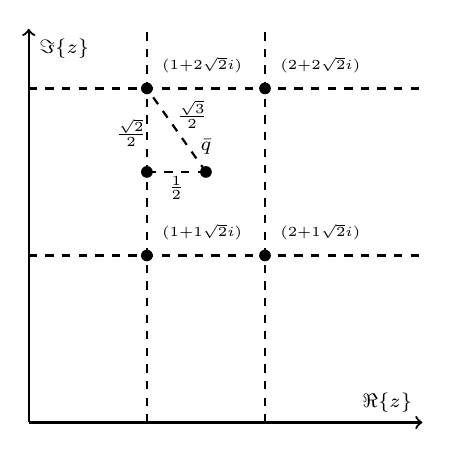
\begin{tikzpicture}
	%XY Axes
    \begin{scope}[thick,font=\scriptsize]
    \draw [->] (0,0) -- (5,0) node [above left]  {$\Re\{z\}$};
    \draw [->] (0,0) -- (0,5) node [below right] {$\Im\{z\}$};
    %Nodes
    \edef\c{1.5}
    \foreach \x in {1,2}{%
    \draw [dashed] (\c*\x,0) -- (\c*\x,5);
    \draw [dashed] (0, {\c*\x*sqrt(2)}) -- (5, {\c*\x*sqrt(2)});
    	\foreach \y in {1,2}{
        	\draw ({\c*\x}, {\c*\y*sqrt(2)}) 
        	node[circle,fill,inner sep=1.5pt,label=above right:				
        	\tiny(\x+\y$\sqrt{2}i$)] {};
        }
    }
    \coordinate (center) at (\c*1.5,{\c*1.5*sqrt(2)});
    \draw (center) node[circle,fill,inner sep=1.5pt,label=above: $\bar{q}$]{};
    \draw [dashed] (center) -- ({\c*1}, {\c*2*sqrt(2)}) 
    node [midway, yshift=0.2cm, xshift=0.2cm] {$\frac{\sqrt{3}}{2}$};
    
    \draw [dashed] (center) -- ({\c*1}, {\c*1.5*sqrt(2)})
    node [circle,fill,inner sep=1.5pt] {} 
    node [midway, yshift=-0.2cm] {$\frac{1}{2}$}
    node [yshift=0.5cm, xshift=-0.2cm] {$\frac{\sqrt{2}}{2}$};
    \end{scope}
\end{tikzpicture}
\end{center}
	We can see that the maximal possible distance between $q$ and $\bar{q}$
	is $\frac{\sqrt{3}}{2}$, which means that:
	\[
		|q-\bar{q}|^2 = N(q-\bar{q}) < \frac{3}{4}
	\]
	Now if we define $r = b\bar{q} - bq$ we see that:
	\[
		a = b\bar{q} \Rightarrow bq + r
	\]
	And using the facts from earlier we get:
	\[
		N(r) = N(b\bar{q} - bq) = N(b(\bar{q} - q)) = N(b)N(\bar{q} - q) < 
		\frac{3}{4} N(b) < N(b)
	\]
	As we wanted, which shows that $R$ coupled with $N$ is a euclidean domain.
	
	\newpage
	
	\textbf{
	Let $R$ be a PID, $F$ the field of fractions of $R$, and $A$ a ring such 
	that $R\subseteq A \subseteq F$. We shall think of the elements of $F$ as 
	fractions of the form $a,b\in R$, $[a,b]=\frac{a}{b}$. Show that if $[a,b]
	\in A$ for $a,b\in R$ that are coprime in $R$, then $[1,b]\in A$.} \\
	Let $a,b$ be coprime in $R$. That means that 
	$\langle a\rangle + \langle b\rangle = R$ thus exist $r_1,r_2\in R$ such 
	that:
	\[
		1 = r_1a + r_2b
	\]
	And now since $r_2,r_1\in R$ they are in $A$ as well and now:
	\[
		\frac{a}{b}r_1 + r_2 = \frac{1}{b}(r_1a + r_2b) = \frac{a}{b}
	\]
	Since $A$ is closed under multiplication we know that $\frac{1}{b}\in A$
	
	\newpage
	
	\subsection{Show that $A$ is a PID}
	Let $I \idealin A$, we know that $R \cap I$ is an ideal in $R$ and
	since $R$ is a PID we can look at its generator such that 
	$\langle r \rangle = R\cup I$. We will now show that the ideal 
	$\langle r \rangle_A$ which is the ideal generated by $r$ in $A$ is
	equal to $I$. It's clear that:
	\[
		\langle r \rangle_A \subseteq I
	\]
	Let $[a,b]\in I$, since $b\in A$ that means that 
	\[
		b * \frac{a}{b} = a \in I
	\] 
	but also we know that $a\in R$, so since $\langle r \rangle$ is a prime 
	ideal in $R$ it follows that:
	\[
		\exists r'\in R \colon a = a'r \Rightarrow [a,b] = [a',b]r
	\]
	Since $a',[1,b]\in A$ we see that $[a,b] = [a',b]r \in \langle r 
	\rangle_A$ which shows:
	\[
		I \subseteq \langle r \rangle_A
	\]
	Finally:
	\[
		I = \langle r \rangle_A
	\]
	Which means that $I$ is a prime ideal in $A$ so $A$ is a PID.
	
	\newpage
	
	\textbf{
	Let $F$ be a field of character $0$. A polynomial $f\in F[x]$ is called 
	squareless if there does not exist $g(x)\in F(x)$ of positive degree such 
	that $g^2\mid f$. Show that $f$ is squareless iff $f,f'$ are coprime in 
	$F[x]$} \\
	\underline{$(\Rightarrow)$} \\
	Let $f\in F[x]$ be squareless. Assume that $f,f'$ are not coprime.
	That means that exists $0\neq p\in F[x]$ irreducible and 
	$q_1,q_2\in F[x]$ such that:
	\begin{align*}
		f(x)  &= p(x)q_1(x) \\
		f'(x) &= p(x)q_2(x)
	\end{align*}
	From this follows that:
	\[
		f'(x) = [p(x)q_1(x)]' = p'(x)q_1(x) + p(x)q'_1(x) = p(x)q_2(x)
	\]
	We notice that:
	\[
		p'(x)q_1(x) = p(x)\left(q_2(x)-q'_1(x)\right)
	\]
	So $p \mid p'q_1$, it can't divide $p'$ since its different than $0$
	and $F$ is a field of characteristic $0$ so it must divide $q_1$.
	From this follows:
	\[
		p \mid q_1 \Rightarrow p^2 \mid pq_1 = f
	\]
	In contradiction to the assumption that $f$ is squareless. \\
	\underline{$(\Leftarrow)$} \\
	Let $f,f'\in F[x]$ be comprime, assume that exists $p\in F[x]$ such
	that:
	\[
		p^2 \mid f
	\]
	We know that exists $q\in F[x]$ such that:
	\[
		f(x) = p^2(x)q(x)
	\]
	But differentiating we get:
	\[
		f'(x) = p^2(x)q'(x) + 2p(x)p'(x)q(x)
	\]
	So we got that $p \mid f$ and $p \mid f'$ in contradiction to the 
	assumption that they are not prime.
	
	\newpage
	
	\textbf{Let $R$ be a PID and $\{0\}\neq I\idealin R$. Show that 
	$\bigslant{R}{I}$ has a finite amount of ideals.} \\
	Since $R$ is a PID exists $r\in R$ such that $I = \langle r \rangle$,
	it follows that:
	\[
		\bigslant{R}{I} = \bigslant{R}{\langle r \rangle} = 
		\{
			ar \vert a\in R
		\}
	\]
	From the correspondence theorem for ideals we know that each ideal
	$A \idealin \bigslant{R}{I}$ exists a corresponding ideal 
	$I \subseteq B \idealin R$. Since $R$ is a PID we get that 
	$B = \langle b \rangle$ and now since $I\subseteq B$ it follows that
	$b \mid r$. Since $R$ is a PID it is a UFD, which implies that exist
	$p_1,\dots,p_n$ irreducable and unique of to permutation
	and multiplication in units such that:
	\[
		r = \prod_i{p_i}
	\]
	Which means that $r$ has a finite number of divisors up to associativity
	of the elements, and in fact it has exactly $2^n$ such divisors. From
	the correspondence theorem that means $\bigslant{R}{I}$ has $2^n$ ideals
	if we show that ideals generated by associative elements are equal. But
	that's exactly what we have shown on the first question, so 
	$\bigslant{R}{I}$ has exactly $2^n$ ideals, which is a finite amount.
	
	\newpage
	\section{Fields}
	
	\textbf{Let $\omega$ be an algebraic number of an odd degree over the 
	field $F$ and show that $F[\omega]=F[\omega^2]$} \\\\
	\underline{$F[\omega^2] \subseteq F[\omega]$} \\
	We know that $\omega\in F[\omega]$ so since it is closed under 
	multiplication we get $\omega^2\in F[\omega]$. So now we can generate 
	$F[\omega^2]$ in $F[\omega]$ and as we wanted we get that $F[\omega^2] 
	\subseteq F[\omega]$ \\
	\\ \underline{$F[\omega] \subseteq F[\omega^2]$} \\
	Because we have shown that $F[\omega^2] \subseteq F[\omega]$ we get that:
	\[
		[F[\omega^2] \colon F] \mid [F[\omega] \colon F]
	\]
	Assume that:
	\[
		[F[\omega^2] \colon F] < [F[\omega] \colon F]
	\]
	Since we know $\omega$ is of an odd degree so 
	$F[\omega] \subseteq F[\omega]$ is odd we also get that:
	\[
		[F[\omega^2] \colon F] < \frac{[F[\omega] \colon F]}{2}
	\]
	Denote $[F[\omega^2] \colon F]$ as $n$ and the minimal polynomial of 
	$\omega^2$ as $p(x) = a_nx^n+\cdots a_0$ as see that:
	\[
		p(\omega^2) = a_n\omega^{2n}+\cdots+a_0 = 0
	\]
	This is a polynomial of degree $2n$ with root $\omega$ so we get that:
	\[
		[F[\omega] \colon F] \le 2n
	\]
	Which is a contradiction to:
	\[
		n = [F[\omega^2] \colon F] < \frac{[F[\omega] \colon F]}{2}
	\]
	So we got that:
	\[
		[F[\omega^2] \colon F] = [F[\omega] \colon F]
	\]
	Since we know that $F[\omega^2] \subseteq F[\omega]$ we get that:
	\[
		\boxed{F[\omega^2] = F[\omega]}
	\]
	
	\newpage
	
	\textbf{Let $\theta$ be a complex root of $p(x)=x^3-9x+6$, express 
	$\frac{1}{\theta+1}$ as a rational polynomial in $\theta$} \\
	We want to get:
	\[
		\frac{1}{1+\theta} = \sum_{i=0}^{n}{a_nx^n}
	\]
	If we multiply both sides by $1+\theta$ we get that:
	\[
		1 = \sum_{i=0}^{n}{a_nx^n} + \theta \sum_{i=0}^{n}{a_nx^n}
	\]
	So:
	\[
		a_n\theta^{n+1} + \sum_{i=1}^{n}{(a_n + a_{n-1})x^n} + a_0 - 1 = 0
	\]
	We know that $\theta$ is a root of $p(x)$ so for $n=2$ and some $c$ we get
	that:
	\[
		a_2\theta^3 + (a_2+a_1)\theta^2 + (a_1+a_0)\theta + a_0-1 = 
		c(\theta^3-9\theta+6)
	\]
	This implies that $a_2 = c$ and we also see that:
	\[
		a_2+a_1 = 0 \Rightarrow a_1 = -c
	\]
	And:
	\[
		a_1 + a_0 = -9c \Rightarrow a_0 = -8c
	\]
	And finally:
	\[
		a_0 - 1 = 6c \Rightarrow c = -\frac{1}{14}
	\]
	We now found all the constants we needed so we get:
	\[
		\boxed{
		\frac{1}{1+\theta} = -\frac{1}{14}\theta^3 + \frac{9}{14}\theta - 
		\frac{3}{7}}
	\]
	
	\newpage
	
	\textbf{Calculate the degree and the minimal polynomial of 
	$\alpha = \sqrt{3+\sqrt{2}}$ over $\Q$} \\
	Calculate to get:
	\begin{align*}
		&\alpha = \sqrt{3+\sqrt{2}} \\ 
		&\Rightarrow \alpha^2-2 = \sqrt{2} \\
		&\Rightarrow \alpha^4-6\alpha^2+7=0
	\end{align*}
	Solving for the roots of the equation:
	\[
		m(x) = x^4-6x^2+7 = 0
	\]
	Gives:
	\[
		x = \pm\sqrt{3\pm \sqrt{2}}
	\]
	Since x isn't rational it doesn't split to polynomials of degrees $1$ and
	$3$, but it might split into $2$ polynomials of degree $2$. We will show
	that is not the case. Suppose it could split into two polynomials with
	degree $2$ then each could be written as:
	\[
		q(x) = (x-x_i)(x-x_j) = x^2 -(x_i+x_j)x + x_ix_j
	\]
	For $x_i \neq x_j$ roots we calculated earlier. If the polynomial is
	rational we get that $x_ix_j\in\Q$ but we can see it's not the case
	since for any of the roots there are we get:
	\[
		x_ix_j =
		\left(\pm\sqrt{3\pm \sqrt{2}}\right)
		\left(\pm\sqrt{3\pm \sqrt{2}}\right) = 
		\left\{
			3\pm \sqrt{2}, \sqrt{7}
		\right\}
	\]
	These are all not rational and therefore $q(x)\notin\Q[x]$ so we got that:
	\[
		\boxed{m(x) = x^4-6x^2+7}
	\]
	Does not split any more, which implies it is the minimal polynomial of
	$\alpha$. We may also note that its degree is $4$.
	
	\newpage

	\textbf{Let $p$ be prime. Find the degree of the splitting field of
	$p(x)=x^p-2$ over $\C$} \\
	First we will find the roots over $\C$ like this:
	\[
		x^p = 2
	\]
	So:
	\[
		r^pe^{pi\theta} = 2
	\]
	This means that:
	\[
		r = \sqrt[p]{2} \quad\text{and}\quad \theta \in 
		\left\{ \frac{2\pi}{p}k \right\}
	\]
	For $0 \le k \le p-1$.
	
	\newpage
	
	\section{Practice}
	
	\textbf{Let $R,S$ be rings and $f\colon R\to S$ be a homorphism. Let 
	$I\idealin R$. Show that if $f$ is surjective then $f(I)\idealin S$} \\
	We can see it is a subgroup with regards to addition because if we let
	$f(a),f(b)\in f(I)$ then since $I$ is an ideal $(a-b)\in I$ so
	$f(a-b) = f(a)-f(b)\in I$. Now let $f(r)\in f(I)$ and $s\in S$ since
	$f$ is surjective we know exists $s'\in I$ such that $f(s')=s$ and then
	$f(r)s = f(r)f(s') = f(rs')\in f(I)$ so we got an ideal.
	
	\newpage
	
	\textbf{Give a counter example if we don't require $f$ to be surjective}\\
	We can choose:
	\begin{align*}
		f\colon\Z\to\Q \\
		f(z) = z
	\end{align*}
	And then we can send any ideal for example $\Z$ itself. But $\Z$ is
	not an ideal in $\Q$.
	
	\newpage
	
	\textbf{If $I \{0\}$ is a prime ideal in $R$ then $R$ is integral domain}
	\\
	Suppose $ab = 0\in I$, since $I$ we get $a\in I$ or $b\in I$. But
	since $I=\{0\}$ we get $a=0$ or $b=0$ which completes the proof. \\
	
	\newpage
	
	\textbf{Suppose every ideal in $R$ is prime. Prove that if $a=bc$ for
	$a\neq 0$ then either $b$ or $c$ are units} \\
	Since $\{0\}$ is always an ideal, and in our case it is given to be prime
	we can assume $R$ is an integral domain.
	Let $a=bc$ such that $a\neq 0$. Since we have $bc\in \ideal{a}$
	we get that either $b$ or $c$ are in $\ideal{a}$, WLOG we can assume
	$b = ad$ and then if we substitute this in the original equation
	we get $a=adc$ so we get $a(1-dc) = 0$ but since we know $R$ is an
	integral domain and $a\neq 0$ we have $cd = dc = 1$ which means $c$ is
	a unit.
	
	\newpage
	
	\textbf{We need to show that $R$ is a field} \\
	All that's really left to show is that all the elements are units.
	We can consider the following fact for $a\neq 0$ we have
	$a^2 = aa$, since we are in an integral domain $a^2 \neq 0$ and then
	from the previous exercise we have $a$ is a unit.
	
	\newpage
	
	\textbf{In a Euclidean domain $R$ for every ideal 
	$\{0\} \neq I \idealin R$ there is a finite amount of maximal ideals in
	$\bigslant{R}{I}$} \\
	We know that $R$ is a Euclidean domain so it is a PID which means that
	for every ideal $I \idealin R$ it is generated by an element $a$ which
	means we can write $I = \ideal{a}$ and then from the correspondence
	theorem we have that the ideals in $\bigslant{R}{I}$ are corresponding
	to the ideals that contain $I$ but these correspond to the divisors
	of $a$, and since $R$ as a Euclidean domain is also a UFD we know that
	that number of divisors is finite under associatives and since
	associate elements generate the same ideal, we get that that number
	is finite as needed.
	
	\newpage
	
	\textbf{Let $n \geq 2$ show that $\bigslant{\Z}{\ideal{n}}$ has nilpotent
	elements different than $0$ if and only if $n$ has a prime square in it's 
	factorization} \\
	Suppose $n$ had a prime sqaure in its factorization we would have:
	\[
		n = p^2 r
	\]
	We can consider the element $pr+\Z$ and see that:
	\[
		(pr+n\Z)(pr+n\Z) = (p^2r)r+n\Z = 0+n\Z
	\]
	From the other direction we get that if $\bigslant{n}{\ideal{a}}$ has
	a nilpotent element $b+\Z \neq 0+\Z$ we would have:
	\[
		b^2 = cn
	\]
	For some $c\in\Z$ so we get:
	\[
		b = \sqrt{c}\sqrt{n}
	\]
	If $n$ doesn't have prime squares then $c=nr^2$ which leads to $c \geq n$
	but that can't be the case since $b < n$.
	
	\newpage
	
	\textbf{Let $\Omega$ be a field extension of $F$ and let $a\in\Omega$
	Show that $a$ is algebraic if and only if $F(a)$ is a finite extension
	of $F$.} \\
	If $F(a)$ is a finite extension of $F$ of degree $n$ then we get that:
	\[
		A = \{1,a,a^2,\dots,a^n\}
	\]
	Is linearly dependent so exists a polynomial of degree $n$ with $a$ as
	its root so $a$ is algebraic. If $a$ is algebraic then we can denote
	its minimal polynomial $m$ and now we can show that ?????
	
	\newpage
	
	\textbf{Given a prime number $p$ prove that exists an indecomposable 
	$f(x)\in\Q[x]$ of degree $p$} \\
	We can consider the polynomial:
	\[
		f(x) = x^p - p
	\]
	We can use Eisenstein's criterion to show this satisfies the conditions.
	We see:
	\begin{align*}
		p \mid a_0 = p \\
		p \nmid a_n = 1 \\
		p^2 \nmid a_n = 1
	\end{align*}
	So it is indecomposable.
	
	\newpage
	
	\textbf{Define $\bigslant{L}{K}$ an algebraic extension of $K$.} \\
	$L$ is an algebraic extension of $K$ if for any $a\in L$ exists 
	$f_a(x)\in K[x]$ such that:
	\[
		f_a(a) = 0
	\]
	
	\newpage
	
	\textbf{Let $\Omega$ be a field extension of $\Q$ that contains a root
	for every polynomial in $\Q[x]$. Show that $\Omega$ contains an infinite
	algebraic extension of $\Q$} \\
	
	
	
	
	
	
	
	
	
\end{document}